%\documentclass[11pt,a4paper]{article}


\documentclass{sig-alternate-05-2015}
\usepackage[latin1]{inputenc}
\usepackage{amsmath}
\usepackage{amsfonts}
\usepackage{amssymb}
\usepackage{graphicx}
\usepackage{url}
\usepackage[linesnumbered,ruled]{algorithm2e}
% Copyright
\setcopyright{acmcopyright}
%\setcopyright{acmlicensed}
%\setcopyright{rightsretained}
%\setcopyright{usgov}
%\setcopyright{usgovmixed}
%\setcopyright{cagov}
%\setcopyright{cagovmixed}

\begin{document}
\conferenceinfo{GECCO'17,} {July 15-19, 2017, Berlin, Germany}
\CopyrightYear{2017}
\crdata{TBA}
\clubpenalty=10000
\widowpenalty = 10000

\title{Evolving Evacuation Route Distributions for Urban Areas}

%
% You need the command \numberofauthors to handle the 'placement
% and alignment' of the authors beneath the title.
%
% For aesthetic reasons, we recommend 'three authors at a time'
% i.e. three 'name/affiliation blocks' be placed beneath the title.
%
% NOTE: You are NOT restricted in how many 'rows' of
% "name/affiliations" may appear. We just ask that you restrict
% the number of 'columns' to three.
%
% Because of the available 'opening page real-estate'
% we ask you to refrain from putting more than six authors
% (two rows with three columns) beneath the article title.
% More than six makes the first-page appear very cluttered indeed.
%
% Use the \alignauthor commands to handle the names
% and affiliations for an 'aesthetic maximum' of six authors.
% Add names, affiliations, addresses for
% the seventh etc. author(s) as the argument for the
% \additionalauthors command.
% These 'additional authors' will be output/set for you
% without further effort on your part as the last section in
% the body of your article BEFORE References or any Appendices.

\numberofauthors{2} %  in this sample file, there are a *total*
% of EIGHT authors. SIX appear on the 'first-page' (for formatting
% reasons) and the remaining two appear in the \additionalauthors section.
%
\author{
	% You can go ahead and credit any number of authors here,
	% e.g. one 'row of three' or two rows (consisting of one row of three
	% and a second row of one, two or three).
	%
	% The command \alignauthor (no curly braces needed) should
	% precede each author name, affiliation/snail-mail address and
	% e-mail address. Additionally, tag each line of
	% affiliation/address with \affaddr, and tag the
	% e-mail address with \email.
	%
	% 1st. author
	\alignauthor
	Keith J. Drew\\
	\affaddr{University of Idaho}\\
	\affaddr{895 Perimeter Drive}\\
	\affaddr{Moscow, Idaho 83844}\\
	\email{keithd@vandals.uidaho.edu}
	% 2nd. author
	\alignauthor
	Robert B. Heckendorn\\
	\affaddr{University of Idaho}\\
	\affaddr{895 Perimeter Drive}\\
	\affaddr{Moscow, Idaho 83844}\\
	\email{heckendo@uidaho.edu}
}

% There's nothing stopping you putting the seventh, eighth, etc.
% author on the opening page (as the 'third row') but we ask,
% for aesthetic reasons that you place these 'additional authors'
% in the \additional authors block, viz.
%\additionalauthors{Additional authors: John Smith (The Th{\o}rv{\"a}ld Group,
%	email: {\texttt{jsmith@affiliation.org}}) and Julius P.~Kumquat
%	(The Kumquat Consortium, email: {\texttt{jpkumquat@consortium.net}}).}
% Just remember to make sure that the TOTAL number of authors
% is the number that will appear on the first page PLUS the
% number that will appear in the \additionalauthors section.

	\maketitle
	
	\begin{abstract}
		 We propose a unique evolutionary approach to the problem of evacuating urban areas in preparation or response to disaster events. Our model is unique in design and works for dynamic topologies, different disaster events, and handles roadway congestion. We apply an evolutionary strategy which optimizes traffic flow using static probabilities as traffic distributions - allowing traffic to be directed in a manner which optimizes roadway throughput and human safety, while allowing for route deviation when vehicles do not follow directions. We use a microscopic traffic model that is unconcerned with individual vehicles or routes. Our model is tested using challenging test cases as well as real-world data. Our results are then provided for comparison.
	\end{abstract}
	\section*{Keywords}
	Evacuation Planning; Evolutionary Strategy; Traffic Congestion, Safety Optimization, Traffic Assignment
	\section{Introduction}
	\subsection{describe need for work}
	Disaster events, both natural and man-made, continue to occur, many with no way of preventing them (natural disasters). Mitigating the loss of life from their effects is of paramount importance. To that end, evacuation planning is crucial. If properly managed, evacuations can reduce loss of life as a result of disaster events significantly. Such planning can be effective both in the time leading up to and in response to disaster events. 
	
	\subsection{describe how new technology is providing new opportunities}
	With technological advances in infrastructure and vehicle automation, communication technology such as smart phones, Geographical Information Systems (GIS), and increased computing power, new solutions and approaches toward evacuation of urban areas are becoming possible \cite{yin2004using}, \cite{yu2002highway}. Advanced simulations can allow us to prepare for certain types of disaster events, and other technologies can assist in evacuation in response to disaster events. Current research in this area leverages new technologies that provide real-time information on traffic systems and events, which allows for more advanced modeling and response to emergencies \cite{hamza2008leveraging}.
	
	\subsection{describe shortcomings of current approaches}
	However, many details of disaster response remain unaddressed in the literature. Specifically, current models may account for changes in area topology, traffic congestion, or a moving source of danger, but don't account for all dynamics together. Problems with current approaches stem from the scope of the problem addressed. Many models are designed for a single type of disaster or event, such as a hurricane, or are coarse grained and focus on evacuating large geographical areas. While models exist at fine-grained levels, and for many different behavioural models, no fine-grained model exists which will work for evacuation planning and response, while handling dynamic topologies, events, and human responses. 
	
	\subsection{describe proposed model}
	To develop such a model, an evolution strategy was chosen. Such an approach can provide an efficient, fast, real-time model that is adaptable and can carry forward information to be used in disaster response, in addition to evacuation planning. The model proposed in this paper is a optimization approach, using fine-grained modeling, and does not use an origin-destionation model, allowing for a more robust solution at the traffic level. Further, the model optimizes routing based on a safety function which can be established for any type of disaster event, and is not limited to disasters, but can be used to describe the goals of evacuation or traffic movement, although this paper focuses on evacuation planning and response. 
	
	To increase optimization speed, this model does use coarse-graining. Traditionally, coarse-graining applies to the graph representations, and is used to group geographically similar areas and therefore simplify the traffic model. However, this model uses course-graining for the vehicle population, allowing a fine-grained modeling of the infrastructure. The grouping of agents allows for a significant decrease in computation time, without loss of accuracy. 
	
	\subsection{describe work done}
	The model developed during the course of this research uses evolution strategies to optimize traffic distributions at each intersection in a given topology. The model is composed of three distinct components. First, a grammar used for defining experiments. Second, a simulation for evaluation the fitness of each potential solution. Finally, an evolution strategy that optimizes results of the simulation based on overall safety of the vehicles in the simulation.
	
	\subsection{describe what has been shown}
	The results found using this model show that evolution is a robust approach because of the information discovered in optimization. We show that given an optimized evacuation plan, dynamics of a disaster event and human behavior can be quickly adapted to and re-optimized for. Further, we show that traditional origin-destination modeling is not necessary for evacuation planning and response.
	
%	--- BEGIN OLD COPY ---
%	
%	Our approach allows evacuation routing to be optimized in preparation for disasters, as well as over the course of a disaster event. Our proposed model evolves probabilities that distribute traffic flow through the area being evacuated and optimizes for safety of individuals. Specifically, we propose that probabilities can be used for traffic assignment throughout the area in need of evacuation. These probabilities represent routing, and are evolved as necessary. We will show in this work that evolution of these distributions provides a robust, dynamic solution that can be quickly updated when presented with changes in topology, vehicle distribution, and safety.
%	
%	During a disaster event, the city topology can change quickly and often. Roadways can be washed out, bridges can collapse, roads may become jammed with traffic, and other unseen events can change the routes available. In addition, people being routed can ignore instructions or make decisions based on daily experiences or social cues \cite{nakajima2007disaster}, causing vehicle distributions to behave in a chaotic manner. Furthermore, areas considered safe can and will change in most disasters, especially if the event moves through the area in need of evacuation. Such events include fires, hurricanes, floods, tsunamis, chemical threats, and others CITEME. Our work provides a mechanism for handling the cases where topologies in a city change, and for re-optimization of the updated topology or event. 
%	
%	Previous approaches to evacuation planning and response include warning systems, assignment-simulation, and route-scheduling. Etc. Etc. CITEME
%	
%	Work in evacuation planning is ongoing and includes some evolutionary approaches, such as Ant Colony Optimization (ACO) \cite{yuan2007multi}, \cite{fang2011hierarchical}. Such work applies a point-to-point methodology for discovering optimal routes to safety, which can miss important solutions or fails in events where the destination is unknown. Our approach provides an optimization based on safety, allowing for discovery of unique and non-intuitive solutions.
%	
%	Some difficulties in evacuation planning include trade-offs between time and safety, congestion issues, and communication of direction to evacuees. Our solution allows for fast optimization of evacuation for large populations of travelers by allowing abstraction of groups of individuals through course graining and probability distributions used for traffic assignment. 
%	
%	In our approach, probabilities representing route distributions in intersections are evolved to optimize safety. Safety is calculated by simulating agent traffic through the desired topology for the specified time, and calculating the safety of all agents at the end of the simulation. This allows the discovery of unique solutions, and allows optimization over specified time periods, while also allowing the use of a number of safety functions. The safety function is a map of safety values applied over the topology, which can be generated by any method - this allows for specification of different disaster types.
%	
%	--- END OLD COPY ---
	
	Section 2 discusses our application target, Section 3 discusses related work and necessary background, Section 4 describes the problem we are concerned with in depth, Section 5 describes our proposed model, and Section 6 discusses our experiments and results.
	
	\section{Problem Description}
		\subsection{general problem}
		Disasters continue to happen year after year and as a result effective evacuation plans are necessary to save lives in the event a disaster calls for evacuation. So far, the problem of evacuation is response to a disaster event is not solved. The literature describes many plans for evacuation, ranging from building evacuation, to stadium and traffic system evacuation, but many models have significant limitations ranging from granularity of the model to the times different models apply, which can be pre-emptive planning models, real-time response, or post-event response models. The model proposed here seeks to provide fine-grained traffic assignment for evacuation zones through all the periods of a disaster event, in a fashion that is event-independent, allowing the use of this model for any disaster event that can be described in terms of safe vs. unsafe areas, providing a safety function over a geographic area.

		\subsection{problem facing pre-emptive evacuation planning}
		Many models focus on pre-emptive planning for evacuation in preparation for certain disaster events. For example, in the U.S.A.,  states coordinate large scale emergency management (EM) plans for evacuation, while cities use models specific to their disaster threats \cite{urbina2003national}. One example of this approach is found in Florida state. In Florida, in response to an increase in tropical storms over the course of 2004-2005, Florida state introduced and passed legislation to enhance statewide evacuation planning and categorize evacuation zones across the state. The plans created focused on hurricanes as the prominent threat to Florida, however they were generalized to any event that called for evacuation \cite{florida2017evacplan}. These zones are used to provide an evacuation plan to the general public via a Florida Division of Emergency Management website \cite{florida2017em}. Our proposed model could augment this type of evacuation plan by providing a fine-grained traffic assignment plan, while using the more coarse-grained planned developed specifically for each region across a state.

		\subsection{problem with origin-destination models}
		The models that use origin-destination algorithms to evaluate shortest path routes, even when coupled with multi-objective optimizations adjusting for other factors such as congestion, are limited by a significant factor, namely that each individual vehicle must be tracked discretely and assigned to a path. This implies a large number of individual path objects, which can take a large amount of memory space for simulation, or might be overwhelming in real-time application with thousands of vehicles being tracked. To handle this issue, routing should be done in a generalized manner, which can ignore the individual identities of and routes, and provide a generalized traffic assignment. Such generalized routing may be achieved by using traffic distributions at each applicable location.

		\subsection{congestion problem}
		Another significant issue when evacuating a population is traffic congestion. It is desireable to maximize throughput of the optimal routes out of the evacuation zone, which means preventing too much congestion. Further, if a significant thorofare becomes congested and throughput of that route drops significantly, a real-time response is necessary to prevent further congestion and allow that congestion to dissipate. 

		\subsection{dynamic events problem}
		The dynamic nature of many disaster events presents another problem, specifically for fine-grained modeling. It may be the case that over the course of a disaster some route that has been assigned becomes impassable or otherwise unusable. When the topology of the evacuation zone changes, a real-time response is necessary to re-route traffic accordingly. It should be pointed out that the issue of congestion can be considered a dynamic event problem - the required real-time response for a blocked road and a road that is unusable due to congestion is the same. 

		\subsection{how our model solves these problems summary}
		The approach propsed here attempts to address these problems by providing a fine-grained evacuation model that generalizes traffic assignment through the use of traffic distributions, while managing congestion and dynamic environment through real-time response.	
	
%	\section{Application Target}
%	The work here is being done in cooperation with Michigan State University researchers.
%	
%	During an evacuation event, zones are often pre-established by coordinators, where routing out of the evacuation zones concerns major road systems such as freeways and highways. Views of these roadway systems are broken into fine or coarse networks \cite{gwynne1999review}. Further, the work required to route traffic for all roads in an urban area can be massive and dependent on various factors, such as time of year or day. For example, populations are distributed differently during rush-hour times than work periods or late at night. The distributions are significantly different, such that traffic routing at a micro level varies significantly. Therefore, a viable approach must be adaptable to different population distributions, as well as topologies and events.
%	
%	The model that we propose generates probabilities used for managing traffic at intersections, with those intersections integrated into a larger graph, representative of the area being evacuated. Our work represents traffic flow and decision making as optimal, indicating out model is an optimization model, according to \cite{gwynne1999review}. however, the manner in which our model's results are applied is not a topic of discussion in this paper. We leave the use of this model to future researchers.
%	

	\section{Related Work \& Background}	
	\subsection{evacuation planning is studied}
	Evacuation planning is not a new topic. 
	Previous work has addressed problems varying from room or building evacuation \cite{thompson1995computer}, \cite{gwynne1999review}, \cite{muhdi2006application} to city and regional evacuation \cite{florida2017evacplan}, \cite{cova2003network}, \cite{lu2004capacity}, \cite{nakajima2007disaster}, \cite{urbina2003national}. We are focused on traffic assignment during evacuation, as opposed to building evacuation, but refer to the taxonomy in \cite{gwynne1999review} for describing our model. 
	In \cite{stepanov2009multi}, Stepanov and Smith describe seven phases of evacuation. Our work focuses on phases V-VII. Those phases are (V), movement through evacuation network, (VI) arrival at safety zone, and (VII) verification. In our work we simulate these phases as necessary to find optimized evacuation plans.
	Key concerns regarding evacuation planning include roadway capacity, travel time, and accuracy of modeling. For roadway capacity, much work has been done in modeling congestion issues in \cite{lu2004capacity}, \cite{chiu2004traffic}, \cite{cova2003network}, \cite{deb2002fast}, \cite{dezani2014optimizing}, \cite{stepanov2009multi}, and more. Accounting for capacity is nearly ubiquitous in the evacuation planning literature, as it is crucial for real applications. Modeling travel time can be accomplished in a number of ways, but is often modeling by use of some link-cost formula, typically based on a form of flow-rate estimation combined with applicable constraints, such as a ratio of current capacity to maximum capacity. The other common method for travel time estimation, which involves evaluating the state of the simulation at regular intervals such as in \cite{chiu2004traffic}, is closely linked with the accuracy of the model being used. Models that evaluate state at regular time intervals tend to be more accurate regarding traffic behavior than flow rate estimation models, but are significantly more complex.  
	
	Models can be broken into categories of fine or coarse grained, regarding how accurately the topology being evacuated is represented \cite{gwynne1999review}. Additionally, models can be described as microscopic or macroscopic, as in \cite{bazzan2014evolutionary}, which refers to the accuracy of simulation and traffic modeling. Traffic assignment models tend to use macroscopic models, reducing complexity of simulation, but microscopic models do exist. We use a fine-grained, macroscopic model to achieve accurate routing for complex traffic systems in fine-grained detail, while abstracting minutia regarding driver behavior, with the assumption that our model can quickly re-optimize to adjust for disparate traffic distributions.
	Another area worth mention regards software optimization and decreasing run-time to achieve results more quickly. Coarse-graining the topology of an evacuation zone is an approach used in some cases, and can be effective at reducing run-time, however, it is not appropriate for our goals, and as such our model tends to run faster for optimizations starting with random individuals for evolution. Another approach to reducing run-time, also adopted by \cite{bazzan2014evolutionary}, is to use vehicle grouping. For the relevant experiments we use different group sizes to maximize group size without loss of accuracy, which leads to significant speed-ups. 
	
	\subsection{evacuation planning background}
	Most traffic assignment and routing algorithms use an origin-destination approach for assigning routes. In our work we leverage probabilities to assign traffic according to traffic distributions, but posit that our assignments are in accordance with Wardrop's First and Second Principles, which state that no unused route will be more optimal than the routes actually used, and that no individual can act unilaterally to improve their route, respectively \cite{wardrop1952road}. The main difference between this approach and typical origin-destination approaches is the focus on managing the evacuees as a whole population, as opposed to considering each individual's route.
	
	Shortest path algorithms, such as Minimal Exposure Shortest Path\cite{chiu2004traffic}, k-shortest paths, and Dijkstra's shortest path algorithm are commonly used to identify optimal routes, and have variations with additional constraints added to improve traffic model accuracy.	Stepanov and Smith approach evacuation planning as a multi-objective optimization problem in \cite{stepanov2009multi}. Stepanov and Smith use Integer Programming, combined with a simulation of traffic and the k-shortest path algorithm. 
	
	Evolution has also been used to optimize routes for evacuation planning. Evolutionary approaches include several Genetic Algorithms (GA) \cite{dezani2014optimizing}, as well as Ant-Colony Optimization (ACO) \cite{forcael2014ant}, \cite{zong2010multi} and multi-objective optimization approaches \cite{saadatseresht2009evacuation}.
	
	Saadatseresht et al. suggest that evacuation is a multi-objective optimization problem \cite{saadatseresht2009evacuation}. Their approach is to use NGSA-II \cite{deb2002fast} to assign origin-destination routes optimized for capacity and nearness of safety zones. Their model is fairly similar to the one we propose here, as it optimizes for safety, and also uses macroscopic simulation, focusing on routing over modeling exact vehicle behaviors. 
	Dezani et al. also optimize origin-destination routes using a genetic algorithm that leverages petri net analysis to evaluate fitness \cite{dezani2014optimizing}. Their model is also macroscopic.
	Recent work by Bazzan et al. \cite{bazzan2014evolutionary} leverages a GA-based method for trip assignment, very quickly. Their model is macroscopic and leverages Wardrop's equilibrium \cite{wardrop1952road}. We compare our results with those found by Bazzan et al. below. 
	For a more comprehensive background on the applications of evolutionary computation in evacuation planning, see \cite{muhdi2006application}.
	
%	
%	Attempts have been made at handling roadway congestion using genetic algorithms, as well. Dezani et al. use Petri net analysis as a fitness function in a GA designed to evolve optimal routes for urban traffic, strictly to reduce roadway congestion in real-time \cite{dezani2014optimizing}. Their approach is not multi-objective, and optimizes routes for shortest time. However, their approach still focuses on origin-destination route solutions for individuals, and optimizes for minimization of travel time alone, while our solution focuses on safety optimization, without determining routes for each traveler. 
	
	\section{Proposed Approach}
	Our proposed model uses an Evolutionary Strategy (ES) to evolve sets of static probabilities that provide traffic distributions at intersections throughout urban areas. The sets of static probabilities are evaluated using an agent-based simulation of traffic in an urban area. To provide a fitness score, a safety function is provided and the sum of safety across all agents is evaluated. We suggest that single-objective optimization of safety, with time and capacity constraints can manage roadway congestion and find optimal routing for vehicles by optimizing a safety function that can be representative of any disaster. 
	
	We propose that evolution of static probability distributions is a more robust approach than evolution of point-to-point routes, such as those used in other approaches like ACO, because of the ability to interchange individuals and use agent grouping. Specifically, using a distribution allows us to treat groups as individuals without significant loss of accuracy, providing a decrease in computation time. Further, a distribution permits deviance from traffic assignment for a portion of individuals by not requiring that specific vehicles follow specific routes.
	
	Another benefit of our model is that each optimization carries important information about routing through the topology. Previous optimizations can be used to initialize future optimizations for similar topologies, allowing a decrease in computation time, as we will show. By carrying forward important infomation, new solutions can be converged upon more quickly. This is true for both changes in the city's topology, such as a roadway becoming unpassable, as well as a change in safety function, as we will demonstrate.
	
	In our approach, safety of the entire population is optimized, instead of individual safety. This allows our model to make trade-offs that benefit the population of evacuees as a whole; such trade-offs may not be seen easily by experts or evacuation planners. 
	
	A city topology is provided as a graph, $G$, before evolution begins, which includes an agent distribution, $A$, evolution parameters, and simulation parameters, such as total simulation time, for evacuation. The topology is identical for all evaluations, and when a change in topology or safety is indicated, evolution begins with the new topology, but using the previous, optimized, static probabilities as a seed to the new evolution. The topology, safety function, and all parameters are designated using SLANG, a grammar for specifying the parameters of a simulation.
	
	Each simulation provides a fitness score for the given set of static probabilities, which is used to evaluate the success of the static probabilities as traffic distributions. This process is repeated as necessary.
	
		\subsection{SLANG Grammar}
			A grammar, SLANG, is used to specify evacuation area topology, safety function, and agent distribution, as well as parameters for the evolutionary strategy and simulation of traffic. 
			
			The most important commands are described here, and are used to build the graph that represents the area topology.
			\begin{itemize}
				\item city STRING INT INT\\
				This SLANG command describes some fundamental information about a city topology. The string argument is the name of the city, the first integer argument indicates the number of nodes, and the second integer is the maximum degree of any node in the topology.
				\item node INT INT FLOAT FLOAT FLOAT FLOAT\\
				The node command is used to specify information about a specific node. The arguments are \emph{node\_ID}, \emph{capacity}, \emph{wait\_time}, \emph{safety}, \emph{latitude}, and \emph{longitude}.
				\item edge INT INT FLOAT FLOAT FLOAT FLOAT FLOAT\\
				The edge command creates edges between nodes as specified, and carries the information necessary to determine link travel time. The arguments are \emph{src\_node\_id}, \emph{dest\_node\_id}, \emph{max\_capacity}, \emph{freeflow\_time}, \emph{B}, \emph{Beta}, and \emph{safety}.
				\item agent INT INT INT\\
				The agent command is used to specify where agents begin the simulation. The arguments are \emph{start\_node}, \emph{number\_of\_agents}, and \emph{individuals\_per\_agent}.
			\end{itemize}
		\subsection{Evolution Strategies Algorithm}
			We chose to use an evolution strategy (ES), as our genome consists of sets of probabilities, represented as real numbers. More specifically, our ES was specified as $ES(\mu + \lambda)$. We compiled results with varying parameters and the best performers are presented. Typically, $\mu = 100, \lambda = 100$ was sufficient, with $\sigma = 0.1$, and with as few as 100 maximum generations for most tests. 
			
			Using the $+$ operator, the child population competes against the parent population for survival. This is performed using a simple sort operation, followed by removal of individuals with the lowest $\lambda$ fitness scores.
			\subsection{Operators}
			\subsubsection{Selection}
			Selection is performed using classic tournament selection, with a tournament of size three. Three random individuals are selected from the population and from those three the one with the highest fitness is selected. Tournament selection helps prevent convergence on local optima. 
			\subsubsection{Mutation}
			Mutation is performed by selecting node probabilities to be mutated with a $50\%$ chance. For any node selected, a random edge-probability is chosen to be mutated by adding a random, normally distributed value, with a standard deviation of $\sigma$, typically equal to $0.1$. Once the value is added, all probabilities for the selected node are re-normalized. Typically, mutation probability was set to $0.5$.
			\subsubsection{Crossover} While crossover is not typically used in evolution strategies, we felt it could help more quickly converge on good solutions, especially combined with the $+$ operator. 
			Crossover is performed by iterating over the set of nodes and choosing, with a $50\%$ chance, node probabilities to swap between the parents. This crossover produces two new individuals. Typically, crossover probability was set to $0.2$. 
		\subsection{Encoding}
			Individuals in the ES are encoded as an array of real number arrays. Each sub-array contains a set of real numbers, one for each choice a traveling agent can make at the corresponding node. As an example, a four-way intersection is represented as a set of five probabilities: one probability for each directional option (say, North, East, South, West), as well as an additional probability to stay in the intersection. All probabilities in a node are normalized to $1.0$. This means an additional operation is required during mutation.
			
			Using real numbers to represent distribution of traffic at a node is useful because they are easily interpreted. Also, by providing a probabilistic distribution, the model works to capture and mitigate events of agent disobedience, where an agent is directed along one path, yet choses a different path. 
				
		\subsection{Simulation}
			During simulation agents move through the provided topology, according to the current set of probabilities being evaluated. Agents are stored in a priority queue, sorted by time of next arrival. All agents start the simulation in a SLANG specified location.
			
			During the simulation, the next agent to be evaluated is selected from the beginning of the priority queue. The agent's next move is determined by selecting an edge to travel along according to the set of probabilities at the agent's current location. After selection, the time of arrival at the agent's next destination is calculated based on edge properties, and the agent is placed back into the priority queue at the appropriate position. This cycle is repeated until the next agent in the priority queue has an arrival time that exceeds the total simulation time, at which point the simulation ends.
			
			\subsubsection{Simulation of Agent movement}
				An agent's selection from the priority queue represents the arrival of that agent at its destination, and there are several possible outcomes. The agent's arrival time may exceed the simulation time, in which case the simulation ends. Otherwise, a random value between 0 and 1 is chosen and the agent's "next node" is selected based on that value. We use a priority queue (which sorts using heapsort) to sort agents in order of arrival time.
				\vspace{3mm}\\
				\includegraphics[width=\linewidth]{sim_diagram.png}\\
				\vspace{3mm}\\
				If the agent "chooses" to remain in its current location, the next arrival time is specified in the SLANG file as a fixed number; the value is the node's \emph{wait\_time}. If the agent chooses a neighboring node as its destination, the next arrival time of the agent is calculated and the agent is placed back in the priority queue. At this point, the next agent is selected and the process is repeated. 
				
				The advantage of using a priority queue sorted by arrival times is that idle time is optimized out of the simulation. In the case of simulating by use of interval-based evaluations, a significant amount of time might be spent performing computations unnecessarily. In some cases, time intervals may be better, but we find this approach more appropriate.
				
				The algorithm for simulation is presented below.
			\subsubsection{Movement}
				Movement of agents through the graph is based on the time is takes to move from one node to another, or how long an agent will wait at a node before making a decision on where to move, and by edge selection when leaving a node with multiple edges. Edge selection is based on the probabilities representing the genome, and is stochastic in nature. The psuedo-code is described below. Travel time between nodes is dictated by the following formula:
				\begin{equation}
				t = f + b(\frac{c}{c_{max}})^{\beta}
				\end{equation} \cite{Horowitz1991}
				where $t$ is the time it costs for an agent to travel an edge. $f$ is freeflow time of the link, which is the time required to travel the link in ideal conditions (typically meaning no other traffic). $c$ is the current capacity of the link, while $c_{max}$ is the maximum number of vehicles that the link can handle per unit time. $b$ and $\beta$ are tuning variables used to fit real data measured from actual roadways. For our purposes we used the default values of $b = 4.00$ and $\beta = 0.15$.
				
				CITEME 
				
				It is important to note that $c_{max}$ is taken to be $2000$ in many applications of this formula, as a default. However, it varies on different roadways, and real-world applications should specify this value appropriately in all uses. 
				
				Some cases of variance in $c_{max}$ include reducing the value based on behavior of traffic lights. For instance, the value is reduced from $2000$ by a proportion equivalent to the proportion of "green time" the traffic light receives at the connected intersection.
				
				It is also important to note that the link cost formula does not include explicit distance or speed limit values, as those values are implied by the freeflow value, $f$, as a result of $t = \frac{distance}{speed}$. 
				
				Additionally, the proposed model specifies hours as the unit of time, as hours are most fitting for the problem domain. 
				
				Algorithm \ref{fitness} describes edge selection.
				
				\begin{algorithm}
					\label{fitness}
					\SetKwInOut{Input}{Input}
					\SetKwInOut{Output}{Output}
					\Input{A set of probability-edge pairs corresponding to a given node}
					\Output{The edge selected}
					
					$random\_value := random(0, 1)$\\
					$probability\_sum := 0$\\
					\ForEach{pair}
					{
						$probability\_sum$ $+=$ $pair.probability$\\
						
						\If{$random\_value < probability\_sum$}
						{
							return $pair.edge$
						}
					}
					\caption{Selects an edge from set of edges who have probabilties that sum to 1.0. Selects according to the probability distribution \emph{on average}, but is stochastic.}
				\end{algorithm}
			\subsubsection{Fitness Evaluation}
				Once the simulation is complete, the set of probabilities used in the simulation are evaluated for their fitness. This is a sum over all the agents for their safety value, given by the safety of the location they are at when fitness is evaluated, in this case at the end of the simulation. The maximum safety for any location in the graph is $1.0$. This leads to the following fitness formula:\\
				\begin{equation}
				f = \frac{1}{n}\sum_{i = 0}^{n} S(a_i)
				\end{equation}
				with n agents, $a$, and safety function $S$. The safety function is simply the safety value of the location the given agent finished the simulation at. This formula returns a fitness value between $0$ and $1$.
				
				This fitness function was chosen to allow adaptability to any disaster event. The differences in how safety is measured between different types of disasters makes using some models unfit for certain types of disasters. However, with this model safety can be designated by any factor. For example, a flood or tsunami event might measure safety as both distance from the event, as well as elevation. An earthquake may quantify safety as distance from tall structures or other hazards. Some events will use distance alone, but other events may have more complex safety functions.
			\subsubsection{An Evaluation}
				In summary, a full fitness evaluation is computed as follows:
				\begin{enumerate}
					\item \textbf{\textit{Initialization}}\\
					The set of probabilities to be evaluated is loaded into the city topology; the city has been defined in SLANG prior to any fitness evalations and the set of probabilities much match that topology.\\
					Agents are initialized in their starting locations and times; their initialization values are specified in SLANG before any fitness evaluations are made. Typically, agents are initialized with an \emph{arrival\_time} of zero seconds.\\
					Finally, the \emph{curr\_time} is set to zero seconds. This value is replaced with each next agent evaluated, and is replaced with the next agent's $arrival\_time$.
					\item \textbf{\textit{Simulation}}\\
					The main activity during simulation consists of popping agents from the priority queue one at a time, evaluating their next move and the arrival time at the next node, and replacing them in the priority queue at the appropriate location. In the case where an agent chooses to stay in a node, the agent's next time of arrival is specified by the node's \emph{wait\_time} field, and is generally fixed.
					\item \textbf{\textit{Fitness}}\\
					The fitness of the set of probabilities is calculated when the simulation time has expired, using equation \ref{fitness}.
				\end{enumerate}
			Here is the psuedo-code:
			\begin{algorithm}
				\SetKwInOut{Input}{Input}
				\SetKwInOut{Output}{Output}
				
				\underline{Simulate}(Chromosome c)\;
				\Input{A set of probabilities for each edge connected to each node; a chromosome}
				\Output{Sum of agent safeties at the end of the simulation, divided by the number of agents}
				\emph{Initialize Probabilities}\\
				\emph{Initialize Agents}
				
				\While{$current\_time < simulation\_time$}
				{
					$agent := priority\_queue.\textbf{pop()}$\\
					$current\_time := agent.\textbf{get\_arrival\_time()}$\\
					
					\If{current\_time > simulation\_time}
					{
						\emph{break}
					}
					
					$current\_node := agent.\textbf{next\_node()}$\\
					$next\_edge := \textbf{choose\_edge(} current\_node \textbf{)}$\\
					
					$agent.\textbf{set\_from\_node(} current\_node \textbf{)}$\\
					$agent.\textbf{set\_current\_edge(} next\_edge \textbf{)}$\\
					$next\_node := next\_edge.\textbf{get\_next\_node()}$\\
					$agent.\textbf{set\_next\_node(} next\_node)$\\
					
					\eIf{$current\_node == next\_node$}
					{
						$t := current\_node.\textbf{get\_wait\_time()}$
					}
					{
						$t := next\_edge.\textbf{get\_traversal\_time()}$
					}
				
					$agent.\textbf{set\_arrival\_time(} current\_time + t \textbf{)}$\\
					$priority\_queue.\textbf{push(} agent\textbf{)}$
				}
			
				\For{$agent_i$ in $priority\_queue$}
				{
					$sum\_safety$ $+= agent_i.\textbf{get\_current\_safety()}$
				}
					
				return $sum\_safety / num\_agents$
				
				\caption{Simulation of agent movement through a defined city topology, based on probabilities provided in Chromosome object}
			\end{algorithm}
		
		
	\section{Experiments}
		Numerous experiments were carried out during development to test the software and ensure the model works as proposed. The experiments discussed here are those related to showing the ability of the model to handle dynamic environments and those used for comparison to other work.
		
		
		zzzSubjecttoChangezzz
		The experiments performed include (1) an experiment to show our model handles changes in topology quickly and accurately; (2) an experiment to show our model handles changes in safety functions quickly and accurately; (3) an experiment to show our model handles changes in agent distribution quickly and accurately; (4) a recreation of the experiment(s) performed in \cite{bazzan2014evolutionary}, for the sake of comparison.
		
		\subsection{Validation Tests}
		To validate our model we needed to test that capacity and freeflow constraints effected our results. To do this we created a simple test with a 5x5 grid, with all edge and node variables equal, and agents initialized to begin in the top left corner of the grid, while safety was only in the bottom right of the grid. After recording the path to safety indicated by highest probabilities, we modify the freeflow values for one test and the capacity for another test. In the case of both tests, we encourage discovery of the same path, but in the first case we do that by greatly reducing the freeflow time of the edges along the selected path, while increasing freeflow along every other edge in the graph, in hopes that the designated path is found by our model. To test capacity constraints, we greatly increase maximum capacity along the selected path, while decreasing maximum capacity along all other edges, in hopes that the designated path is discovered by our model. The following image indicates the indicated path, which was discovered in both cases. Data indicating time to discover from random initialization is included.
		
		First, the results from the baseline test indicates the route most often converged upon by our model. The vehicle traffic flows from along the indicated route: 0, 5, 10, 15, 20, 21, 22, 23, 24. 
		
		\includegraphics[width=\linewidth]{maze_default_solution.png}

		Next, for freeflow validation, we describe a path through the grid that has a freeflow time of INSERT TIME USED HERE across all edges of the path and in the direction of safety and uses freeflow time of INSERT TIME HERE for all other edges. The path discovered is the designated path: 0, 1, 2, 3, 8, 13, 12, 11, 10, 15, 20, 21, 22, 23, 24.
		
		\includegraphics[width=\linewidth]{maze_two_flow_cap.png}
		
		Nexts, the same path is designated for capacity testing, and the results are similar. A maximum capacity of INSERT CAPACITY USED HERE is used for all edges along the path, while a maximum capacity of INSERT CAPACITY USED HERE is used for all other edges in the grid. The designated path is discovered again by our model: 0, 1, 2, 3, 8, 13, 12, 11, 10, 15, 20, 21, 22, 23, 24.
		
		\subsection{Comparison}
		Here we compare our results to results of other tests suited to our model in the literature. Specifically, we are concerned with the work Bazzan et al. \cite{bazzan2014evolutionary}. In their paper, Bazzan et al. seek to minimize average travel time by evolving traffic assignments through a graph, given a set of vehicles, OD pairs for those vehicles, and a set of $k$ shortest paths. They use a classic graph from \cite{willumson2001transport}, with the freeflow times specified there as well. The way we model capacity is different, but comparable. We seek to compare our results to provide some context of how our model holds up compared to other work.
		
		In their experiment they run $k$ OD pairs, with $k$ ranging from two to 16, and we choose to compare to the case where $k=4$. We run our experiment with two vehicle origin nodes, corresponding to their origins, with two safe nodes, corresponding to their destinations. We let our model optimize for safety, and provide the results and comparison below.
		
		Our model is not as optimal, and our average time to complete all traffic is significantly lower. This is probably due to an inconsistency in modeling, but is an area for future study and analysis. While our model does find routes to safety, the routes found are not as fast as those found by Bazzan et al.
		
		The average time to safety (TTS), with standard deviation is show below. 
		
		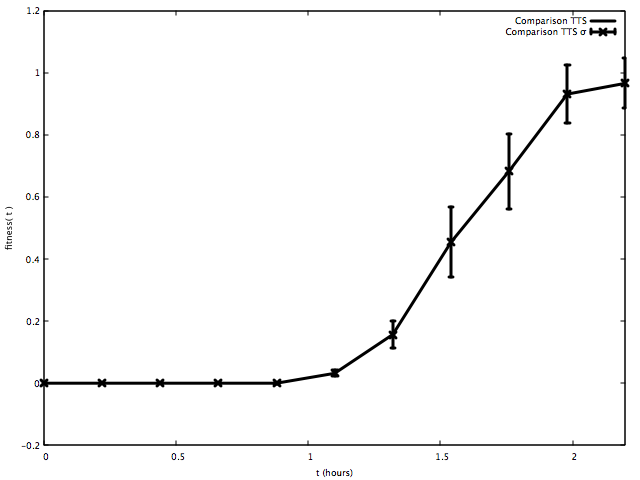
\includegraphics[width=\linewidth]{bazzan_tts_graph.png}
		
		\subsection{Changes}
			The following experiments are carried out in similar fasion and test if our model accommodates dynamic events during an evacuation. We hypothesize that if traffic assignment probability distributions are optimized in advance, they can be used to initialize an evolution strategy to reduce optimization time, both in real time, and number of generations without loss of accuracy. The results of these tests demonstrate that pre-optimization leads to faster adaptability in response to real-time events.
			
			For these experiments we make several assumptions. First, we assume changes are not significantly large. We posit that some pre-computed solutions adapting to changes will be dealing with the smallest changes possible for optimization. If a significantly large change in any characteristic we are investigating occurs, in a fashion too fast to re-optimize solutions for at smaller intervals, re-optimization may not perform better than optimization from a random restart. In fact, and perhaps a matter of future investigation, in such a case where the graph characteristics have been changed significantly, re-optimization using a previous solution may take longer than using random initialization.
			
			The events we are concerned with here involve changes in topology, safety zones, capacity, and vehicle distribution. To test our hypothesis, we perform two initial optimizations (1) we optimize a population of solutions that are initialized with random values for the initial graph configuration and (2) we optimize a population of solutions that are initialized with random values for the graph configuration after some change in topology, safety, capacity, or vehicle distribution has been modified. Finally, we use the final population from the first optimization to initialize the starting population used to optimize the second graph configuration. Results are tabled below.
			For each test, the evolution parameters were kept the same for the sake of an easier comparison. The parameters are $ES(100+100), P_{crossover}=0.2, P_{mutation}=0.5, \sigma=0.1$

			\subsubsection{Adapting to Capacity Changes}
			During an evacuation event a roadway may see a change in capacity as a result of becoming partially blocked by debris, traffic stopping in one or more lanes on a multi-lane road, or as a result of other unpredictable events. In such a case our model must be able to quickly adapt, and we predict that using pre-optimized traffic assignment distributions will allow for quick adaptation. To test this prediction we run three tests. First, we create a topology with a maximum capacity of 1000 vehicles per unit time for all edges, $G_1$. Next, we create a topology that is identical, except that maximum capacity is lowered by 100 for each edge, $G_2$. We then optimize both of these graphs using our models and record the average number of generations until maximum fitness is achieved. We also store the solutions found from $G_1$, as they will be the starting population for optimization in the next test. For the third part of the test we re-optimize $G_2$, starting with the solutions from $G_1$. We record and compare the number of generations needed to reach maximum fitness below. We also show the average time to safety (TTS) of each test, as well as the test topology.
			
			
			\subsubsection{Adapting to Topology Changes}
			Another event that might occur during an evacuation is a change in topology, meaning some route or partial route becomes unusable, such as a bridge collapsing or a road becomes completely blocked by debris. It is important that our model handles such changes quickly. We make a similar prediction to the capacity change test as well, and note that a change in topology is a more extreme version of a change in capacity where maximum capacity is reduced to zero for a roadway. We again run three tests. The first test is on $G_1$, which represents three bridges connecting two areas, with safety being on the side opposite where vehicles are started for these tests. $G_2$ for this test is identical to $G_1$, except with an edge on the center "bridge" removed. The first two graphs are optimized from random traffic assignment probabilities and generations until maximum fitness is acheived are recorded. We then use the solutions from the optimization of $G_1$ to optimize $G_2$, and record the number of generations for comparison. We again show the results and topology below.
			
			\subsubsection{Adapting to Vehicle Distribution Changes}
			In an evacuation event being managed at a fine-grained level, it is expected that individual drivers will, in some cases (if not all) use their own judgement, and ignore directions based on their experience driving in the area. This is expected because optimal traffic assignments may produce non-intuitive results. In such cases, we must again be able to adapt and adjust based on where vehicles actually are. This is particularly important as optimization results from the volume of traffic being routed and should a significant portion of that volume change location, it is crucial to re-optimize for the best chances at reaching safety. We make a similar prediction here - our model will find an optimal solution faster if initialized with a pre-computed solution for a similar traffic distribution. Again, we use three tests. All tests use an identical topology, but $G_1$ has traffic distributed differently than $G_2$. The first two runs optimize for different traffic distributions, starting with randomized traffic assignment probabilities. The third run uses the optimized traffic assignment probabilities from the first test, but with the traffic distribution of the second run. We again record the number of generations until maximum safety is reached, and report the results below. 
			
			\subsubsection{Adapting to Safety Changes}
			During many evacuation events, the threat creating the need for evacuation is often not static. Examples include hurricanes, floods, tsunamis, and more. As a result of the dynamic nature of the threat, it is imperative that our model handles changes in safe areas quickly. We predict here that our model handles changes in safety quickly, again provided the change is not too great. Three runs are used to perform this experiment. The first and second are again identical in topology, with the exception that the safe nodes move over one node from the first run to the second run. The optimized traffic assignment probabilities from run one are used to initialize the third run, which has safety in the same location as run two. The average number of generations required to find maximum fitness are recorded and tabled below. 
			
			
			\subsubsection{Results}			
			The graph shows the safety over time for the agent population. The table shows the average number of generations needed to reach the maximum safety with standard deviation, the average fitness reached with standard deviation, and the total simulation time. All averages were computed over a sample size of 100 runs of the same test. 
			
\includegraphics[width=\linewidth]{composite_tts_graph.png}
%			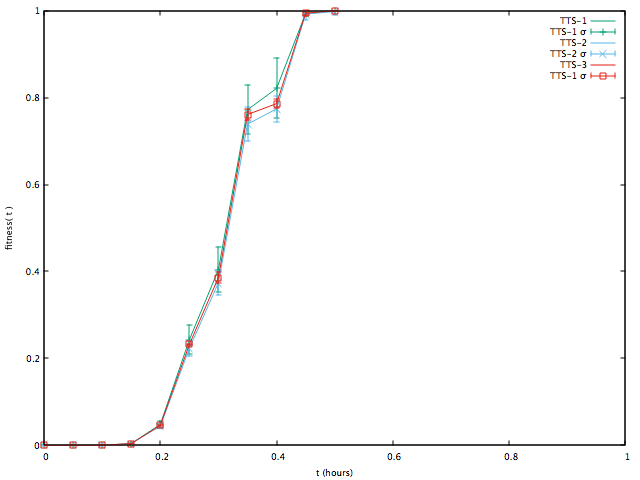
\includegraphics[width=\linewidth]{topology_tts_graph.png}
%			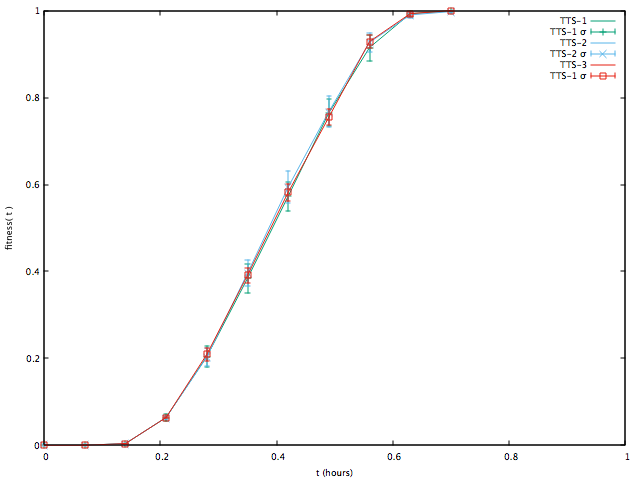
\includegraphics[width=\linewidth]{agents_tts_graph.png}	
			
			\begin{tabular}{l*{6}{c}}
				\hline \hline
				Test & Avg. Gens & $\sigma_{gens}$ & Avg Fit & $\sigma_{fit}$ & $t_{hours}$ \\
				\hline
				Agents1 & 77.99 & 9.605 & 0.999 & 0.003 & 0.7 \\
				Agents2 & 89.69 & 8.577 & 0.998 & 0.004 & 0.7 \\
				Agents3 & 30.5 & 8.325 & 1.0 & 0.0 & 0.7 \\
				\hline
				Capacity1 & 47.75 & 5.208 & 1.0 & 0.0 & 1.0 \\
				Capacity2 & 55.1 & 6.64 & 1.0 & 0.0 & 1.0 \\
				Capacity3 & 4.35 & 2.19 & 1.0 & 0.0 & 1.0 \\
				\hline				
				Safety1 & 43.02 & 8.359 & 1.0 & 0 & 1.0 \\
				Safety2 & 40.855 & 8.2 & 1.0 & 0 & 1.0 \\
				Safety3 & 34.5 & 4.574 & 1.0 & 0 & 1.0 \\
				\hline
				Topology1 & 73.54 & 15.835 & 1.0 & 0.001 & 0.5 \\
				Topology2 & 69.92 & 13.9 & 0.998 & 0.009 & 0.5 \\
				Topology3 & 7.01 & 4.574 & 1.0 & 0.0 & 0.5 \\	
				\hline
			\end{tabular}
		
		\subsection{Boise, Idaho}
			To test the ability of our model to handle real-world urban evacuation problems we used geographical data from Boise, Idaho. As the data we used was less precise than we would like, some assumptions and liberties were taken. First, we don't know the exact freeflow rates of all the roads, nor the maximum capacities of each roadway. However, our goal is to discover how long it takes to optimize solutions for a large problems with large numbers of vehicles. Our data includes 283 nodes, and 914 edges. These do not represent every road and intersection, but our model's runtime is a function of the number of vehicles in the graph, not the size of the graph, so for our purpose here, missing some of the roadways is acceptable. 
			We test a number of cases with varying numbers of vehicles and groups. Each test has a group of ten vehicles initialized to start at every node in the graph. These agents are placed here to ensure probabilities at every area of the graph are optimized. In our model, if an area of the graph sees no traffic, the probabilities at that area are not punished or rewarded which produces random traffic assignments. This affect could have dangerous results in real-world application.
			The tests we run for Boise start with only the single groups of ten vehicles at each node, and scale up to 102,830 vehicles, with large grouping, over five tests. Each test is run with identical evolution and graph values, except where the vehicles are initialized. Vehicle initialization is random, except for the ones forced to start in each node. Each test is run 10 times and the time to run is averaged over those runs. The results are tabled below.
			
			\begin{tabular}{l*{4}{c}}
				\hline \hline
				Agents & Rand Groups & Group Size & Run Time (min)  \\
				\hline
				2,830 & 0 & 10 & 3.5 \\
				2,930 & 10 & 10 &  3.28 \\
				3,830 & 10 & 100 & 3.5 \\
				12,830 & 100 & 100 & 4.4 \\
				102,830 & 100 & 1000 & 4.25 \\
				1,002,830 & 1000 & 1000 & timehere\\
				\hline
			\end{tabular}
		
			These tests were performed with a simulation time of one hour. The runs were performed using Centos 7 VM running with 10 Intel Xeon 5000 processors and 132 GB of RAM. However, the model does not use any multithreading, so multiple processes were spawned to allow us to aggeregate data over many runs.
			
			
%			To test our hypothesis for each type of event, we created unique experiments for each. Here are descriptions and graphs for each.
%			
%			To test if a change in capacity was easily adapted from pre-computed solutions, we use use a graph with 25 nodes in the form of a 5x5 grid. The graph is connected as pictured in FIGURE REF. The edges in the graph all carry a maximum capacity of 1000 vehicles per hour. For the change in capacity, the second graph is identical in all things except that maximum capacity is dropped to 500 vehicles per hour. Finally, the solution found when capacity was at 1000 vehicles per hour is used to optimize the graph with maximum capacity of 500 vehicles per hour. We predict a significantly faster optimization time when using the initial optimized solution population to seed optimization in the second graph.
%			
%			To test if a change in safety was easily adapted from pre-computed solutions we used a simple graph, with a safety plateau in one region of the graph. All edges and nodes in the graph carry equal values, except for the safety plateau. For the first and second optimizations, the safety area is shifted by half of its area through the graph, to represent a moving event, as opposed to a completely new event. Our hypothesis suggests similar optimization times for these two cases. 
%			Next, the second graph is optimized using solutions from the first graph's optimization. Our hypothesis predicts a significant reduction in optimization time for this experiment.
%			
%			To test the hypothesis regarding a change in topology, a new graph is used, which provides a simplified version of a series of bridges. For the change in topology one "bridge" is destroyed. The simulate destruction of the bridge, the pair of edges creating the link between nodes along the bridge are simply removed. We again predict that solutions found in the initial optimization of the first graph will lead to faster optimization of the second graph.
%			
%			To test if a change in vehicle distribution is easily adapted from pre-computed solutions, we use the graph used for testing capacity and safety. All edges and values describing the behaviour of the graph and traffic flow are identical between each other. The only safe area in the graph is found at node 24, which acts as a sink for vehicles, representing escape from danger. Vehicles are initialized in nodes 0 and 1, 1000 vehicles in each, for a total of 2000 vehicles, for graph one. In the second graph the vehicles are initialized in the top right corner and the bottom left corner, 1000 vehicles in each corner. We test our hypothesis regarding change in vehicle distribution by again optimizing each variation of the graph from initially random populations. Then we re-optimize the second graph using the first set of optimizations and compare the time needed to optimize.

	\section{Conclusion}
		In conclusion, evolved static probability distributions are shown to provide routing to safe areas in reasonable time. Further, the solutions used are provided as initializations for topology changes, which reduce the optimization times of the updated topology. These changes carry forward important routing information, already found in previous optimizations, while adapting around the changes. The main advantages of our proposed model include systems for managing a dynamic topology and vehicle distribution, relatively fast computation time, and robustness achieved through both evolution and a vehicle distribution model, instead of point-to-point routing for individual agents.
		
		\subsection{Future Work}
		\begin{itemize}
			\item Optimization including threading
			\item Risk and threat assemssment
			\item Novel application specific operator research
			\item Visualization
			
		\end{itemize}
		
	\section{Acknowledgments}
	Folks at MSU\\
	Anton Stalick\\
	Homaja Marisetta\\
	Other relevant work.
	
	\bibliography{mybib}
	\bibliographystyle{IEEEtran}
	
	\section{extra}
			\subsection{Exhaustive Search}
	To get an idea of what the fitness landscape looks like for problems in the evacuation space according to our model look like, we performed an exhaustive search on a three-node problem. Our graph was very simple, and the search consisted of exploring the probabilities with precision of two decimals, for two nodes, labeled $x$ and $y$, with fitness on the $z$ axis. The topology:\\
	\includegraphics[width=\linewidth]{exhaustive_diagram.png}
	with both node zero, one, and their edges having $0.0$ safety, and node two having a self-edge with safety $1.0$.  Using an agent population of $5000$ with all agents starting on node zero, the fitness landscape is seen in the following image:\\
	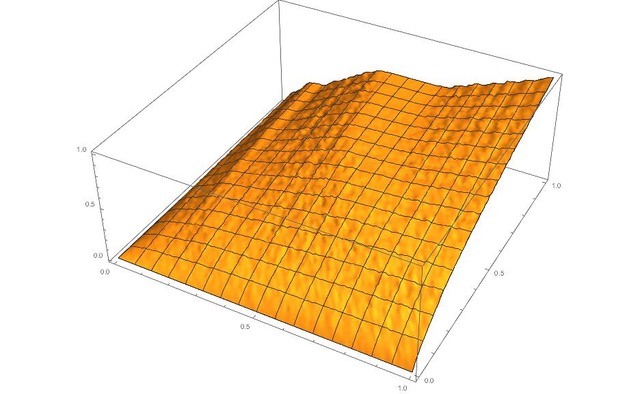
\includegraphics[width=\linewidth]{exp-avg-10.jpeg}\\
	It is important to note that for each probability pair $(x,y)$, the simulation was run 10 times and the fitness for each run was averaged. This provides smoothing, which is helpful because of the stochastic nature of edge selection.
	
	\subsection{Validation Tests}
	To confirm that evolution was optimizing safety, we developed a set of simple tests. These are specified in SLANG, and are very simplified.
	\begin{itemize}
		\item \textbf{pit.slang} The pit test describes a 10-node graph, with a middle node and two outer rings. Safety is lowest in the center and highest on the outer ring. Our algorithm optimizes the probabilities so that agents are pushed toward the other ring. See results below
		
		\includegraphics[width=\linewidth]{pit_diagram.png}
		INSERT RESULT DATA HERE
		\item \textbf{maze1.slang} The first maze test sought to evaluate how probabilities were optimized given a safety path through a grid. The grid was 5x5 and the path of safety saw nodes and edges along path increase gradually from zero safety to maximum safety. This test produced very different results depending on how much time was given for optimization. 
		
		\includegraphics[width=\linewidth]{maze_1.png}
		INSERT RESULT DATA HERE
		\item \textbf{maze2.slang} The second maze produced logically similar results to the second maze, but was forced to handle congestion conflicts differently because of the safety path. 
		
		\includegraphics[width=\linewidth]{maze_2.png}
		INSERT RESULT DATA HERE
		\item \textbf{bridges.slang} bridges is used to verify that solutions can be found more quickly with pre-optimized probability sets when the topology is changed. In the bridges test, first an optimization is performed on the following graph, with agents beginning in the left-most column, and safety found in the right-most column. 
		
		\includegraphics[width=\linewidth]{bridge1.png}
		After an optimization was found, the probabilities and number of generations to find a solution were saved. Next, the same graph is optimized from random probabilities, but with an edge removed representing a bridge collapse. 
		
		\includegraphics[width=\linewidth]{bridge2.png}
		The number of generations to find a solution from random probabilities is again saved. Finally, the second topology is re-optimized, but with the optimal set of probabilities from the first optimization (with the bridge in tact) added into the population of solutions. The optimization is run, and the number of generations again recorded.
		
		\includegraphics[width=\linewidth]{mPeaks.png}
		INSERT RESULT DATA HERE
		\item \textbf{dSlope.slang} dSlope is a test with a deceptive slope. The same 5x5 grid is used, but with a safety gradient that is deceptive. Safety rises towards one corner of the grid and in the corner there is a drop-off in safety to zero. However, the opposite corner holds the peak, with a maximum safety value. In this test, probabilities found the peak with randomized agent starting locations where some of the agents started near the peak, but failed to find the peak if agents started too far from it. However, the solution did optimize safety well in the cases where it couldn't find the peak. 
		
		\includegraphics[width=\linewidth]{dSlope.png}
		INSERT RESULT DATA HERE
		\item \textbf{highway.slang} The highway test was used to see if our model found solutions based on time. One possible path allows agents to travel on a highway with a low freeflow time. The other possible routes have a much higher freeflow time. This test was to see if, with a large agent population, a solution that utilized both paths could be found. Such a solution was found, accounting for congestion. 
		\begin{center}
			\includegraphics[scale=0.5]{highway_diagram.png}
		\end{center}	
		INSERT RESULT DATA HERE
		\item \textbf{grid.slang} The grid test is used to verify that solutions can be found more quickly with pre-optimized probability sets when the given safety function changes. In this test an optimization is performed on two similar safety functions, as shown, with randomized initial probabilities. For each, the number of generations required to arrive at an optimal solution is recorded. In these tests, agents begin along the top row of nodes.
		
		\textbf{safety1:}
		
		\includegraphics[width=\linewidth]{safety1.png}
		
		\textbf{safety2:}
		
		\includegraphics[width=\linewidth]{safety2.png}
		
		After the optimizations are recorded, the set of probabilities found for the first safety function are used in the initialization of the probability population of the second safety function, and the number of generations required to find an optimal solution are recorded. 
		INSERT RESULT DATA HERE
	\end{itemize}
	
	\subsection{Anaheim, California}
	To test a realistic optimization, Anaheim, California was chosen, as data was readily available, and an initial SLANG specification was available from previous work. 
	
	Traffic data provided by the City of Anaheim, available online \cite{anaheim2016data} was used as a basis for agent distribution, and tests were performed over rush-hour traffic times.
	
	The Anaheim example is used to test two ideas. First, we wanted to test that our model can provide an optimization for a large, real-world example. Second, we wanted to test the feasibility of handling changes in topology quickly. We propose that an optimal set of static probabilities used for initialization of a different, yet similar, topology would reduce the optimization time of the updated topology. We believe that the reduction in time is proof that the body of information in our solutions is carried through evolution, and propogated forward. 
	
	First, an optimization of traffic is performed with agents starting in the North-West area of Anaheim, and a safety plateau in the South-East area of Anaheim, allowing for use of I-5 through the city by agents travelling towards the "safe-zone". The optimization runs for [insert time here] and is initialized with random static probabilities.
	
	Next, an edge along the I-5 path is removed from the graph, and the optimization is perfomed again. All parameters are the same as for the previous optimization, save the missing edge, which makes the I-5 route partially unusable. Removing an edge of the major thorofare should prove to be a significant difference, one which affects the movement of traffic in the simulation.
	
	Finally, the second optimization is performed again, but initialized with the set of probabilities produced from the first optimization. This optimation should complete faster than the second optimization which had to start with random static probabilities. 
	
	RESULTS
\end{document}